\begin{frame}{Code Generation}
  % Code Generation Example as TikZ diagram, matching provided screenshot
  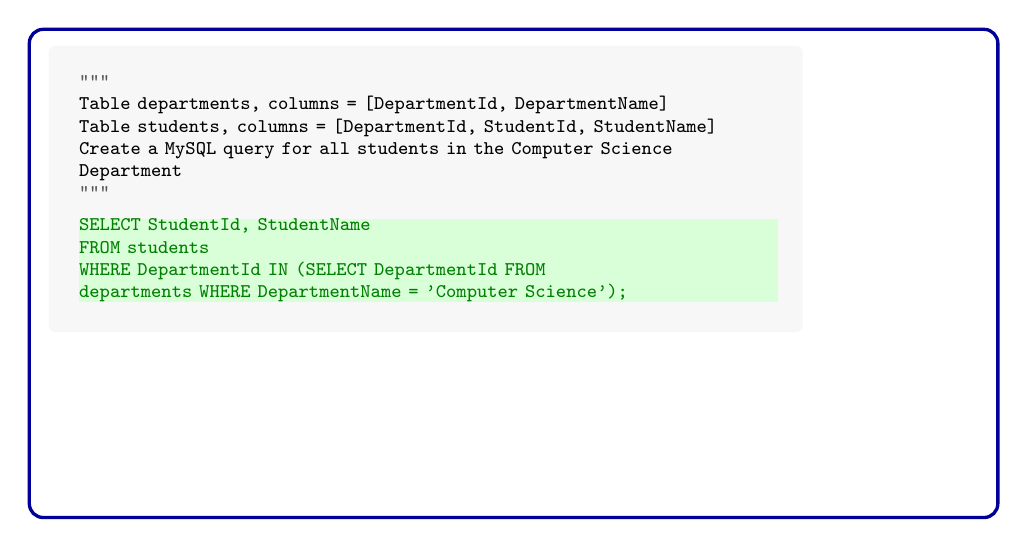
\begin{tikzpicture}
    % Outer rounded rectangle with blue border
    \node[draw=blue!60!black, very thick, fill=white, rounded corners=5pt, minimum width=12.3cm, minimum height=6.2cm, anchor=north west, inner sep=0pt] (outline) at (0,6) {};


    % Text block: verbatim prompt and query, matching screenshot exactly
    \node[anchor=north west, font=\ttfamily\scriptsize, text width=8.8cm, align=left, fill=gray!6, rounded corners=2.5pt, inner sep=1.1em, xshift=0.26cm, yshift=-0.22cm] (textbox) at (outline.north west) {%
\textcolor{gray!70!black}{\texttt{"""}}\\
\texttt{Table departments, columns = [DepartmentId, DepartmentName]}\\
\texttt{Table students, columns = [DepartmentId, StudentId, StudentName]}\\
\texttt{Create a MySQL query for all students in the Computer Science Department}\\
\textcolor{gray!70!black}{\texttt{"""}}\\[0.5em]
\setlength{\fboxsep}{0pt}%
\colorbox{green!15!white}{%
  \parbox[t]{\dimexpr\linewidth-0.01cm}{%
    \textcolor{green!50!black}{\texttt{SELECT StudentId, StudentName}}\\
    \textcolor{green!50!black}{\texttt{FROM students}}\\
    \textcolor{green!50!black}{\texttt{WHERE DepartmentId IN (SELECT DepartmentId FROM}}\\
    \textcolor{green!50!black}{\texttt{departments WHERE DepartmentName = 'Computer Science');}}
  }
}
    };
  \end{tikzpicture}
\end{frame}
